% DO NOT COMPILE THIS FILE DIRECTLY!
% This is included by the other .tex files.

\begin{frame}[t,plain]
\titlepage
\end{frame}

\begin{frame}
    \frametitle{Example of use-cases}
    \begin{itemize}
        \item \textbf{Notification} on specifc actions
        \begin{itemize}
            \item New events matching criteria
            \item New users
            \item Automated alerts for high-priority IOCs
        \end{itemize}
        \item \textbf{Extend} existing MISP behavior
        \begin{itemize}
            \item Push data to another system
            \item Automatic enrichment
            \item Sanity check to block publishing / sharing
            \item Curation pipelines
        \end{itemize}
        \item \textbf{Hook} capabilities
        \begin{itemize}
            \item Assign tasks and notify incident response team members
        \end{itemize}
        \item ...
    \end{itemize}
\end{frame}

% \section{Workflow - Fundamentals}
\begin{frame}
    \frametitle{
        \huge
        Workflow - Fundamentals
        \vspace{1em}
    }
    \textbf{Objective:} Start with the foundation to understand the basics
    \begin{center}
        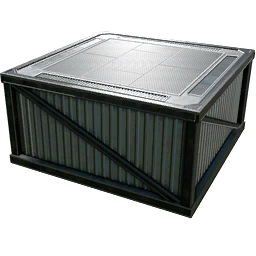
\includegraphics[width=0.07\linewidth]{pictures/fundation}
    \end{center}
\end{frame}

\begin{frame}
    \frametitle{Triggers}
    Currently 11 triggers can be hooked. 3 being 
\includegraphics[width=36px]{pictures/blocking-workflow.png}.
    \begin{center}
        \frame{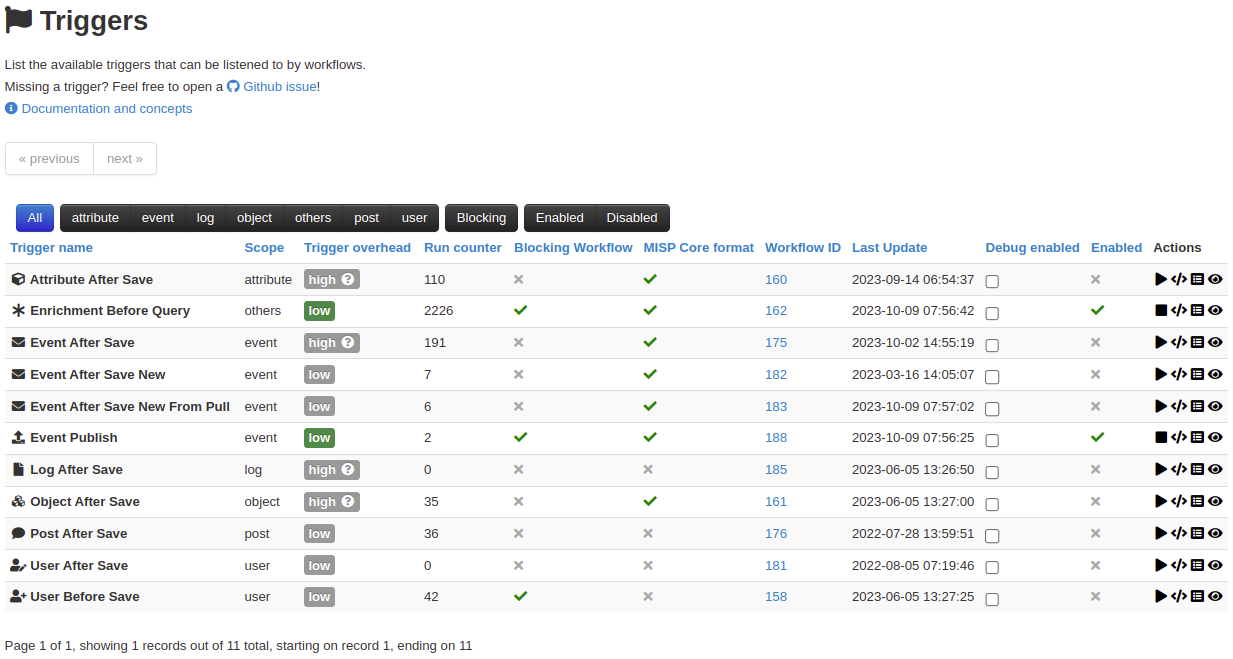
\includegraphics[width=1.0\linewidth]{pictures/triggers.png}}
    \end{center}
\end{frame}

\begin{frame}
    \frametitle{Logic modules / Conditions}
    \vspace*{0.25em}
    
\includegraphics[width=70px]{pictures/sc-condition.png}
    \vspace*{0.25em}
    {\Large \faIcon{question-circle}} \textbf{Logic modules} allow to redirect the execution flow
    \begin{itemize}
        % \colorbox{red!100}{\textcolor{white}{\texttt{tlp:red}}}
        \item A MISP Event is tagged with \texttt{tlp:red}
        \item The distribution of an Attribute is a sharing group
        \item The creator organisation is \texttt{circl.lu}
        \item Or any other \textbf{generic} conditions
    \end{itemize}

    \vspace*{0.5em}
    \begin{center}
        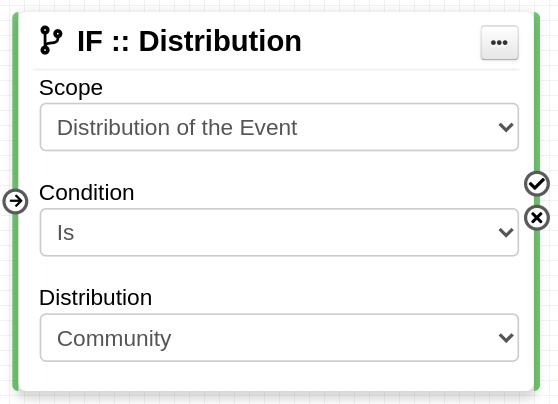
\includegraphics[width=0.43\textwidth]{pictures/logic-module.png}
    \end{center}
\end{frame}

\begin{frame}
    \frametitle{Actions modules}
    \vspace*{0.25em}
    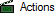
\includegraphics[width=60px]{pictures/sc-action.png}
    \vspace*{0.25em}
    {\Large \faIcon{question-circle}} \textbf{Action modules} allow to executes operations
    \begin{itemize}
        \item Send an email notification
        \item Perform enrichments
        \item Send a chat message on MS Teams
        \item Attach a local tag
        \item ...
    \end{itemize}

    \vspace*{0.5em}
    \begin{center}
        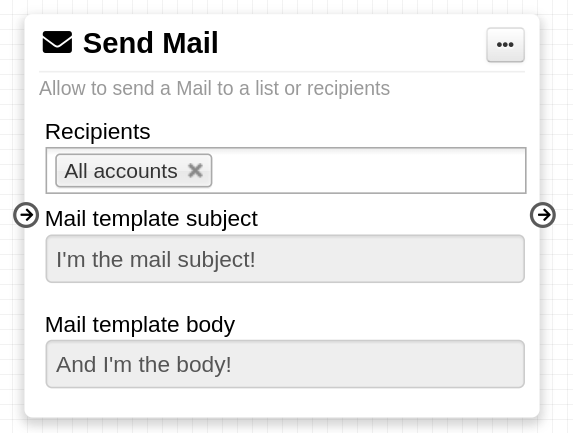
\includegraphics[width=0.43\textwidth]{pictures/action-module.png}
    \end{center}
\end{frame}

\begin{frame}
    \frametitle{What is a MISP Workflow?}
    \begin{itemize}
        \item Sequence of all nodes to be executed in a specific order
        \item Workflows can be enabled / disabled
        \item A Workflow is associated to \textbf{1-and-only-1 trigger}
    \end{itemize}
    \vspace*{0.5em}
    \begin{center}
        \frame{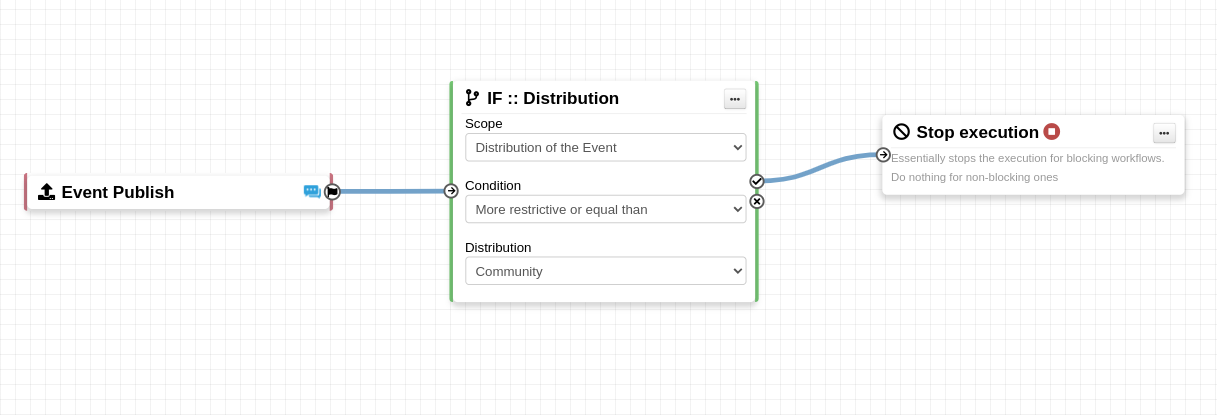
\includegraphics[width=1.0\linewidth]{pictures/simple-workflow.png}}
    \end{center}
\end{frame}


\begin{frame}
    \frametitle{Sources of Workflow modules}
    {\large Built-in \textbf{default} modules}
    \begin{itemize}
        \item Part of the MISP codebase
        \item Ready to use once enabled
    \end{itemize}
    \vspace{1em}
    {\large User-defined \textbf{custom} modules}
    \vspace{0.5em}
    \begin{columns}[t]
        \begin{column}{0.5\textwidth}
            \underline{Written in PHP}
            \begin{itemize}
                \item Extend existing modules
                \item MISP code reuse
            \end{itemize}
        \end{column}
        \begin{column}{0.5\textwidth}
            \underline{Written in Python}
            \begin{itemize}
                \item Can rely on extensive python libraries
                \item Easier to write
                \item Rely on the \textbf{enrichment service} 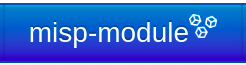
\includegraphics[width=0.12\linewidth]{pictures/misp-module-icon.png}
            \end{itemize}
        \end{column}
    \end{columns}
\end{frame}

\begin{frame}
    \frametitle{Demo by examples}
    \begin{enumerate}
        \item[WF-1.] Send an email to \textbf{all admins} when a new event has been pulled
        \vspace*{2em}
        \item[WF-2.] Block queries on 3rd party services when \textbf{tlp:red} or \textbf{PAP:red}
        \begin{itemize}
            \item \textbf{tlp:red}: For the eyes and ears of individual recipients only
            \item \textbf{PAP:RED}: Only passive actions that are not detectable from the outside
        \end{itemize}
    \end{enumerate}
\end{frame}

\begin{frame}
    \frametitle{Demo WF-1: Send an email to \textbf{all admins} when a new event has been pulled}
     \begin{center}
        \frame{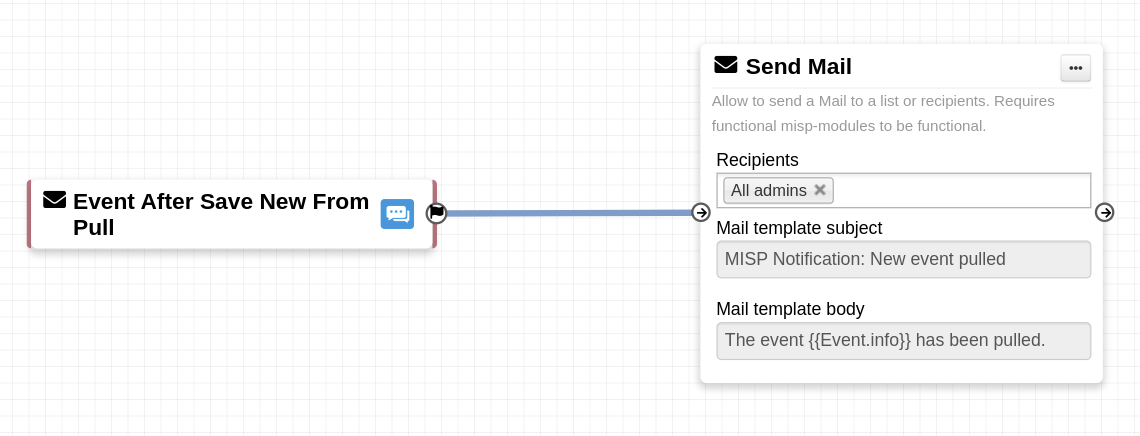
\includegraphics[width=1.0\linewidth]{pictures/demo-wf1.png}}
    \end{center}
\end{frame}

\begin{frame}
    \frametitle{Demo WF-2: Block queries on 3rd party services when \textbf{tlp:red} or \textbf{PAP:red}}
    \begin{itemize}
        \small
        \item \textbf{tlp:red}: For the eyes and ears of individual recipients only
        \item \textbf{PAP:RED}: Only passive actions that are not detectable from the outside
    \end{itemize}
    \vspace*{1em}
     \begin{center}
        \frame{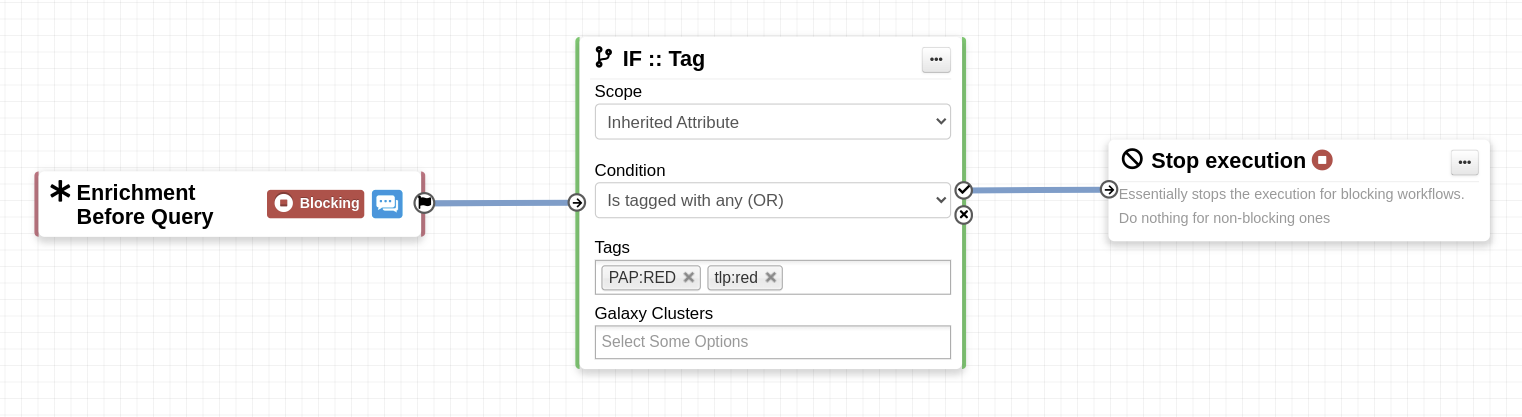
\includegraphics[width=1.0\linewidth]{pictures/demo-wf2.png}}
    \end{center}
\end{frame}

\begin{frame}
    \frametitle{Creating a workflow with the editor}
    \begin{enumerate}
        \item \underline{Prevent} event publication \texttt{\bf \large if tlp:red} tag
        \begin{itemize}
            \item \underline{Send a mail} to \texttt{\scriptsize admin@admin.test} about potential data leak
        \end{itemize}
        \item \texttt{\bf \large else}, \underline{send a notification} on Mattermost
    \end{enumerate}
\end{frame}

% \section{Considerations when working with workflows}
\begin{frame}
    \frametitle{
        \huge
        Considerations when working with workflows
        \vspace{1em}
    }
    \textbf{Objective:} Overview of some common pitfalls
    \begin{center}
        
\includegraphics[width=24px]{pictures/radar.png}
    \end{center}
\end{frame}

\begin{frame}
    \frametitle{Working with the editor - Operations not allowed}
    Execution loop are not authorized
    \vspace*{1em}
    \begin{columns}
        \begin{column}{0.7\textwidth}
            \frame{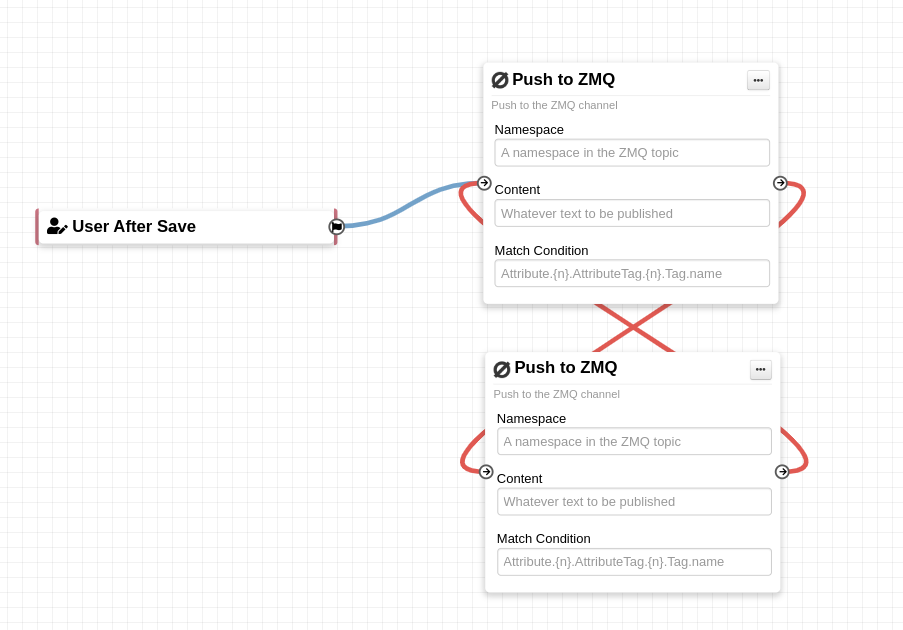
\includegraphics[width=1.0\linewidth]{pictures/editor-not-allowed-1.png}}
        \end{column}
        \begin{column}{0.3\textwidth}
            \frame{
\includegraphics[width=1.0\linewidth]{pictures/infinite-loop.jpg}}
        \end{column}
    \end{columns}
\end{frame}

\begin{frame}
    \frametitle{Recursive workflows}
    \frame{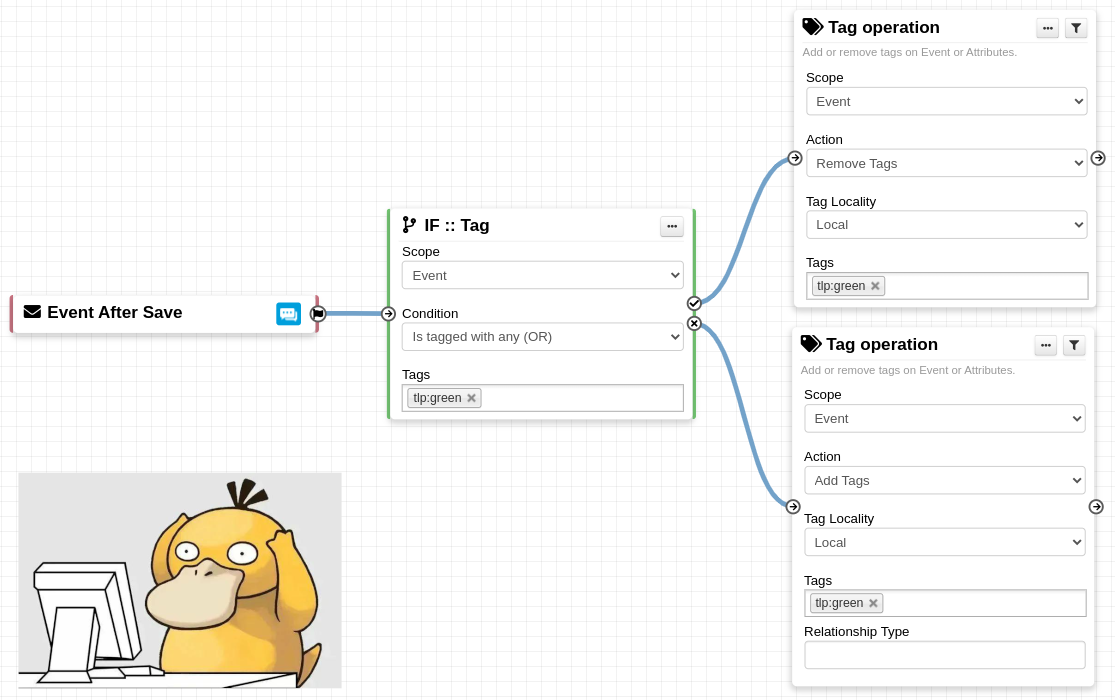
\includegraphics[width=1.0\linewidth]{pictures/recursive-workflow.png}}
    \danger Recursion: If an action re-run the workflow
\end{frame}

\begin{frame}
    \frametitle{Working with the editor - Operations not allowed}
    Multiple connections from the same output
    \vspace*{1em}
    \begin{columns}
        \begin{column}{0.7\textwidth}
            \frame{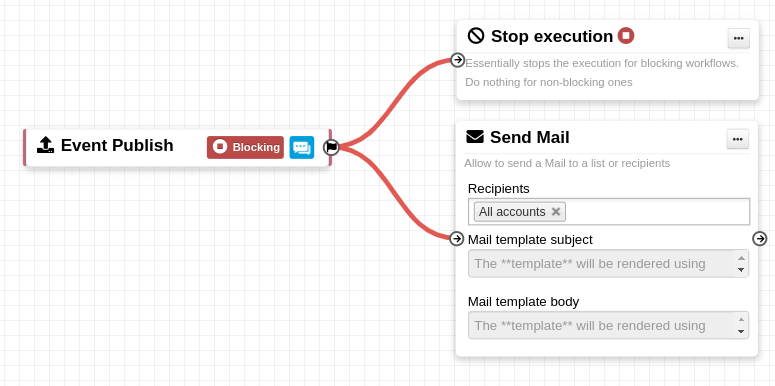
\includegraphics[width=1.0\linewidth]{pictures/editor-not-allowed-2.png}}
        \end{column}
        \begin{column}{0.3\textwidth}
            \frame{
\includegraphics[width=1.0\linewidth]{pictures/two-paths.jpeg}}
        \end{column}
    \end{columns}
    \begin{itemize}
        \item Execution order not guaranted
        \item Confusing for users
    \end{itemize}
\end{frame}

\section{New recent features}
\begin{frame}
    \frametitle{New recent features I}
    \begin{itemize}
        \item New action modules \& improvements
        \begin{itemize}
            \item \texttt{Assign country}
            \item \texttt{Attach warninglist}
            \item \texttt{Attribute operations}
            \item \texttt{Tag replacements}
            \item \texttt{Webhook}, $\cdots$
        \end{itemize}
        \item New logic modules \& improvements
        \begin{itemize}
            \item \texttt{Filter :: Generic}
            \item \texttt{Filter :: Remove}
            \item \texttt{IF :: *}
        \end{itemize}
    \end{itemize}
\end{frame}

\begin{frame}
    \frametitle{New recent features I}
    \frame{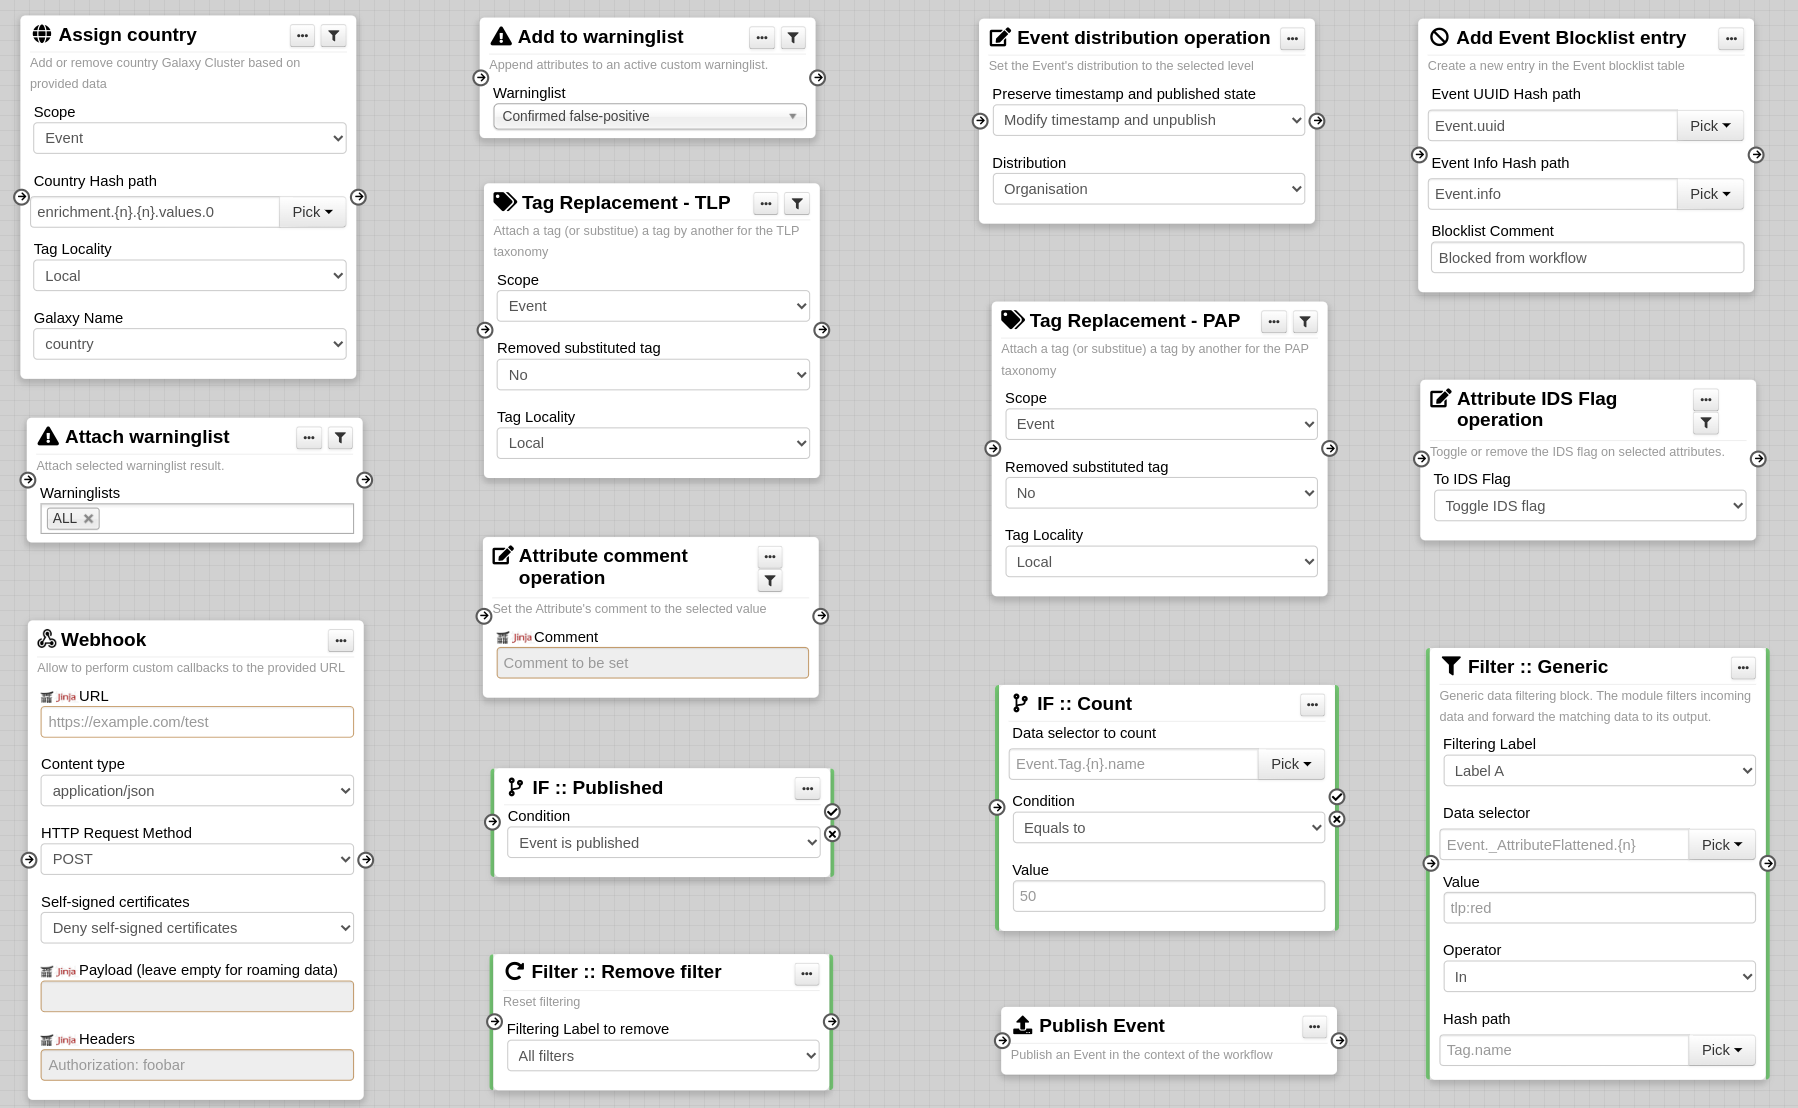
\includegraphics[width=1.0\linewidth]{pictures/new-modules.png}}
\end{frame}

\begin{frame}
    \frametitle{New recent features II}
    $\sim 12$ New blueprints for IoC curation
    \frame{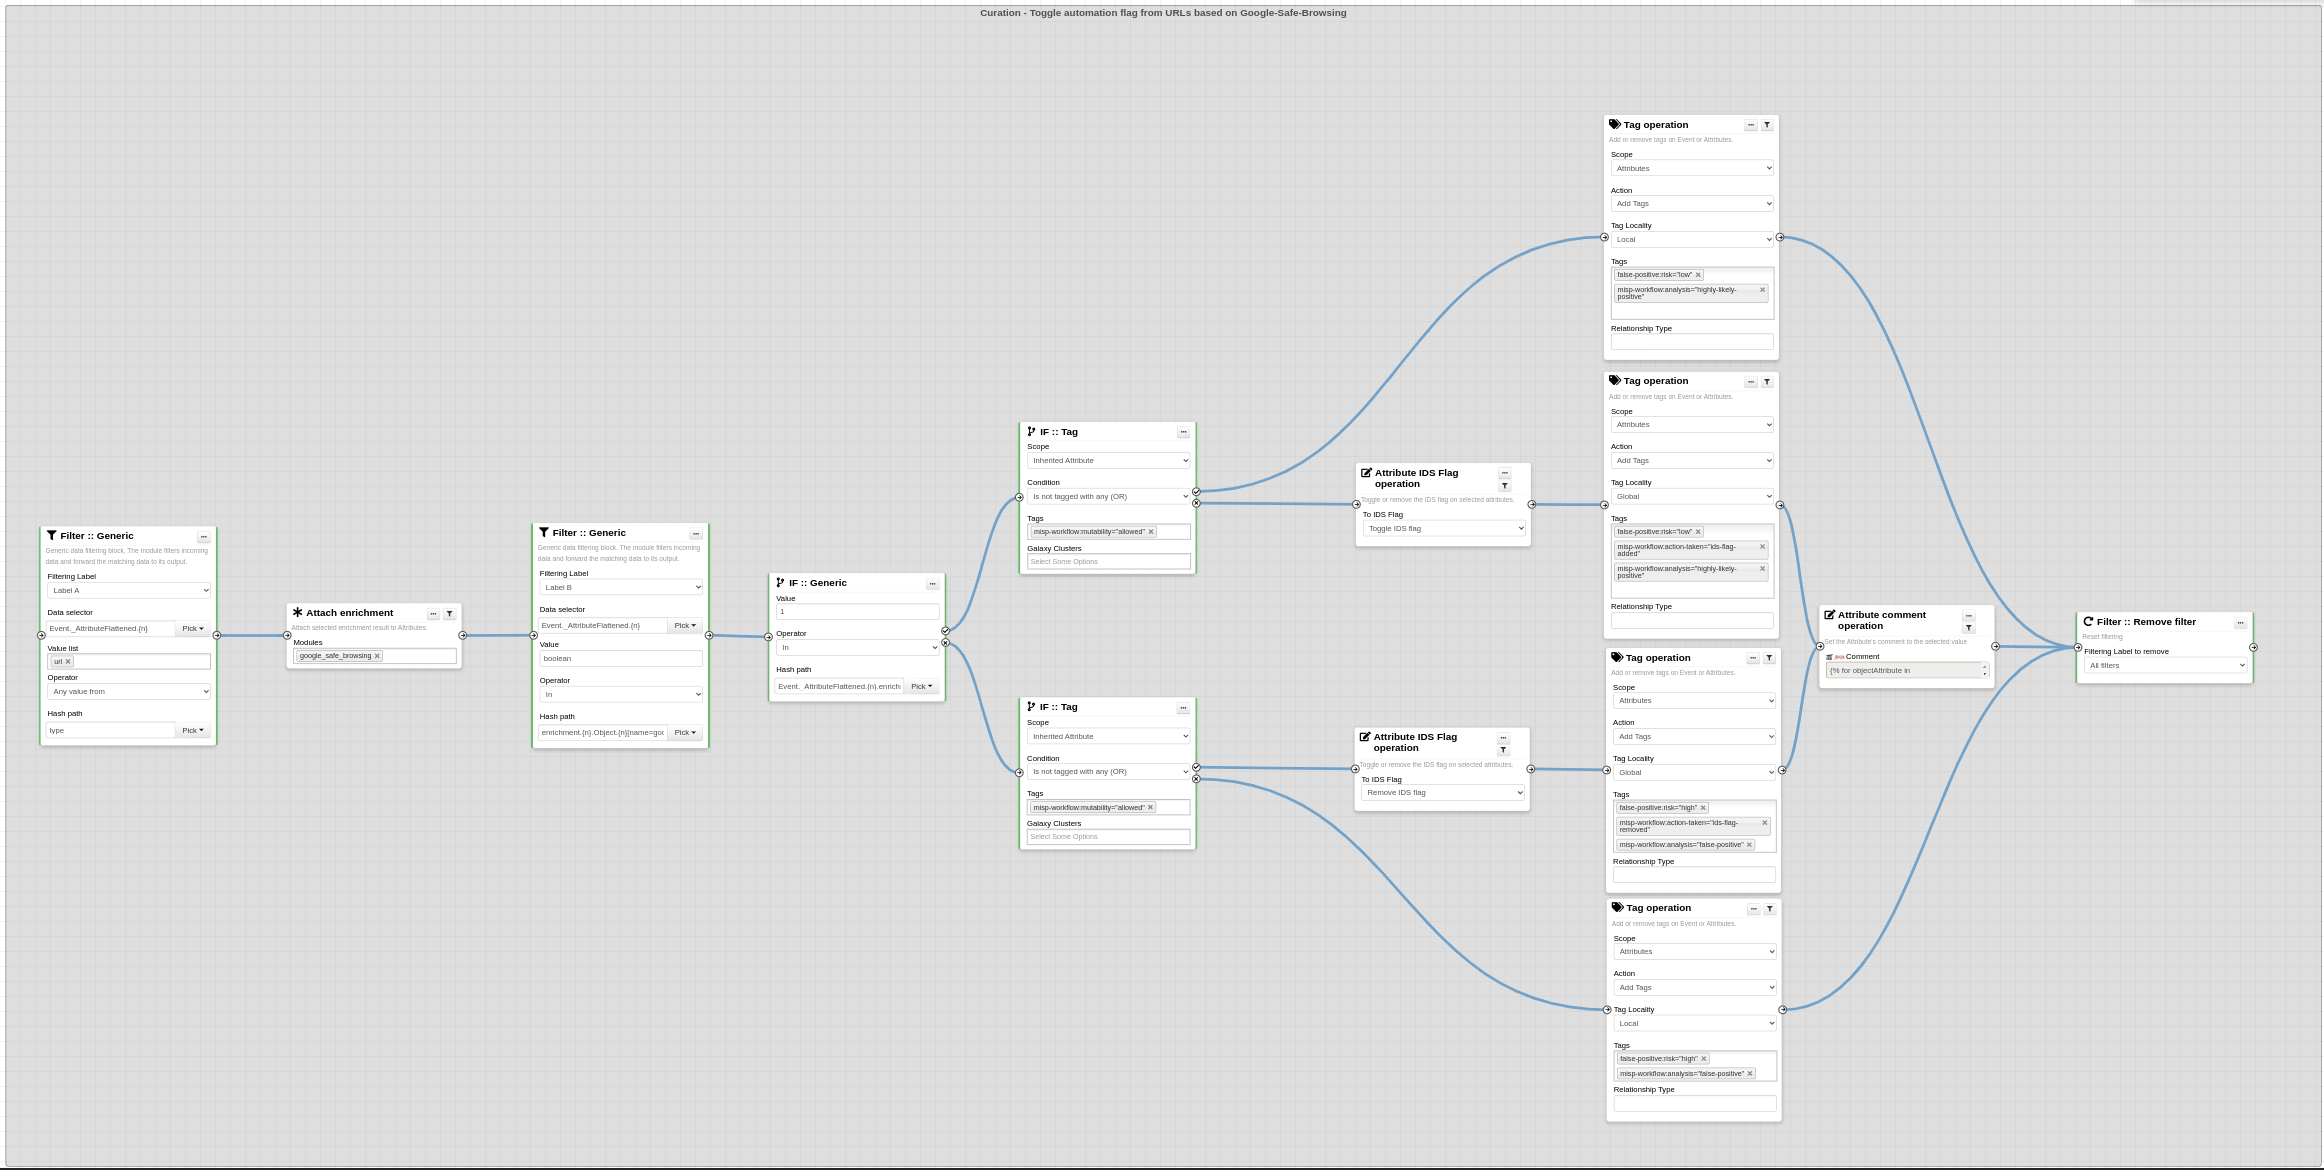
\includegraphics[width=1.0\linewidth]{pictures/curation-google-safe-browsing.png}}
\end{frame}

\begin{frame}
    \frametitle{New recent features III}
    \begin{itemize}
        \item UI improvements
        \begin{itemize}
            \item Frame to annotate and group modules
            \item More documentation (Format, Jinja2 syntax)
            \item Collapsible sidebar and quick node insert
            \item Hash path picker
        \end{itemize}
    \end{itemize}
    \begin{center}
        \frame{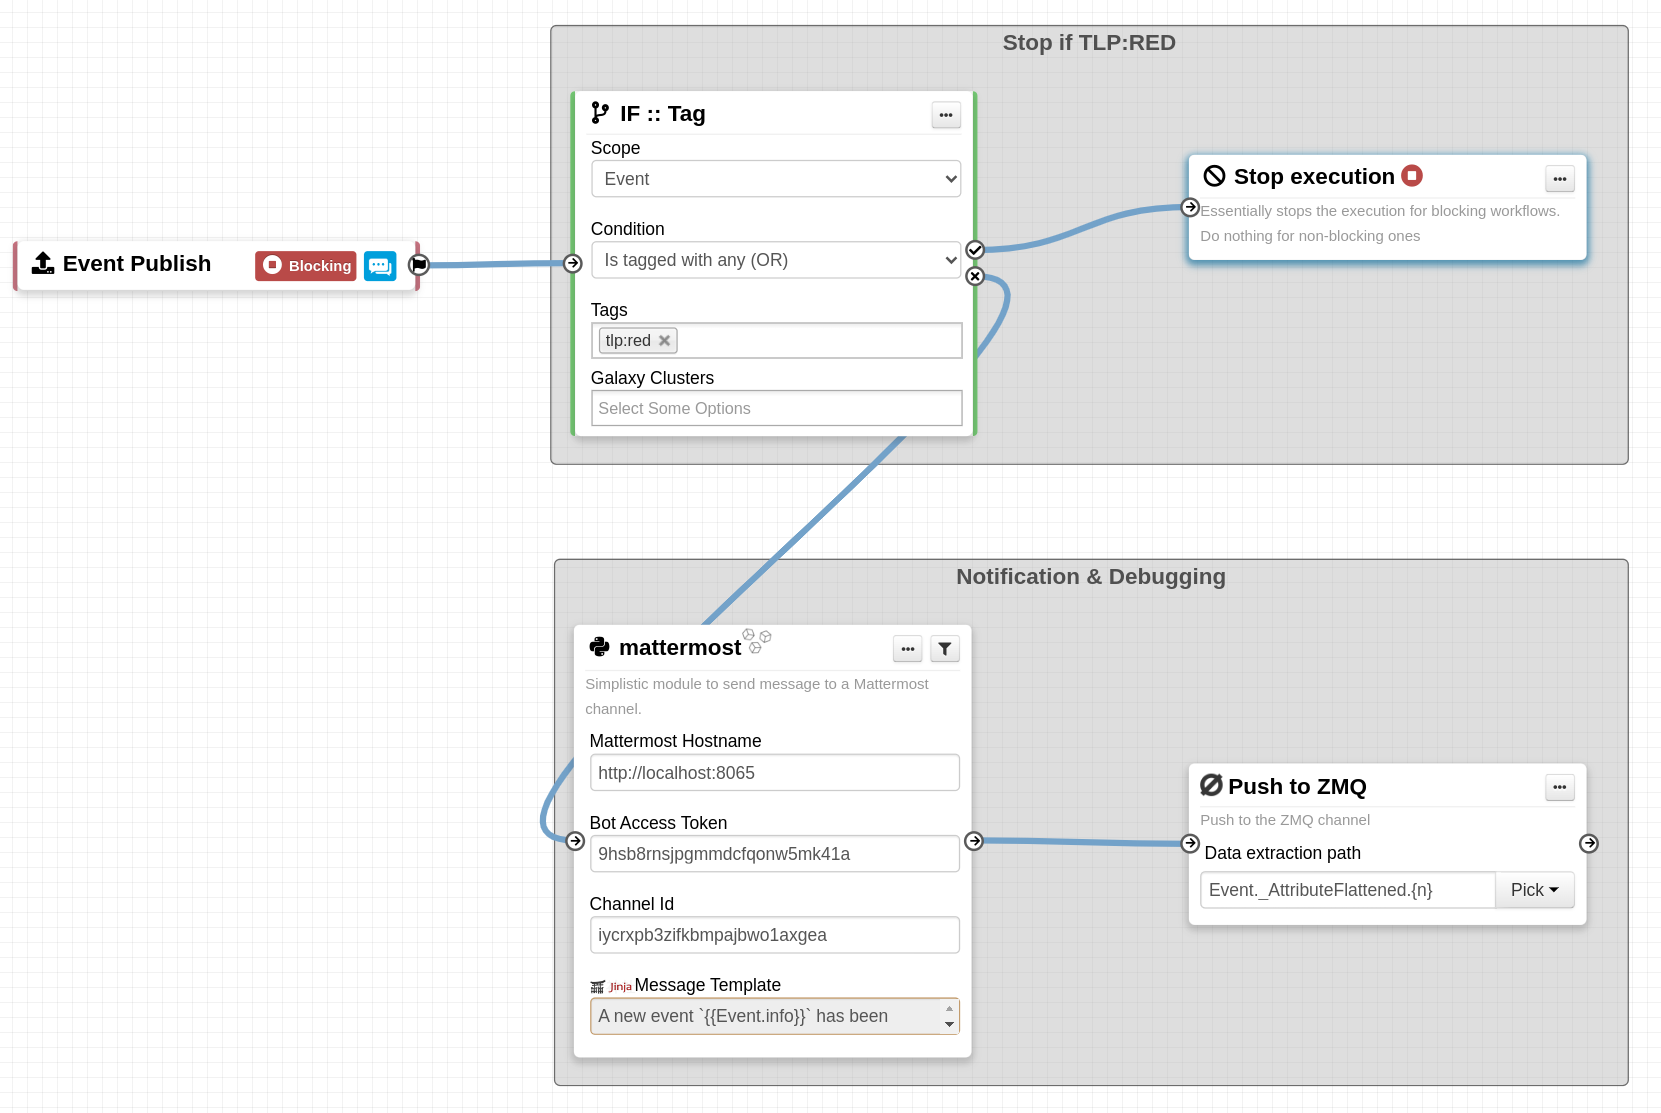
\includegraphics[width=0.7\linewidth]{pictures/frames.png}}
    \end{center}
\end{frame}

\section{Advanced usage}
\begin{frame}
    \frametitle{
        \huge
        Advanced usage
        \vspace{1em}
    }
    \textbf{Objective:}
    \begin{itemize}
        \item Blocking workflows
        \item Blueprints
        \item Filtering
        \item Data format
        \item Debugging
    \end{itemize}
\end{frame}

\begin{frame}
    \frametitle{Blocking and non-blocking}
    Two types of workflows:
    \vspace{0.5em}
    \begin{itemize}
        \item[] \hspace*{-2em}
\includegraphics[valign=m,width=48px]{pictures/blocking-workflow.png} Workflows
        \begin{itemize}
            \item Can prevent / block the original event to happen
            \item If a \textbf{blocking module}
\includegraphics[valign=b,width=12px]{pictures/blocking-module.png} blocks the action
            \item \texttt{event-publish}, \texttt{event-before-save}, \texttt{enrichment-before-query}, $\cdots$
        \end{itemize}
        \vspace{0.5em}
        \item[] \hspace*{-2em}
\includegraphics[valign=b,width=56px]{pictures/non-blocking-workflow.png} Workflows execution outcome has no impact
        \begin{itemize}
            \item No way to prevent something that happened in the past
            \item \texttt{event-after-save}, \texttt{attribute-after-save} \texttt{log-after-save}, $\cdots$
        \end{itemize}
    \end{itemize}
\end{frame}

\begin{frame}
    \frametitle{Logic module: Concurrent Task}
    \begin{itemize}
        \item Logic module allowing \textbf{multiple output} connections
        \item \textbf{Postpone the execution} for remaining modules
        \item Convert 
\includegraphics[valign=b,width=44px]{pictures/blocking-workflow.png} \faIcon{long-arrow-alt-right} 
\includegraphics[valign=b,width=56px]{pictures/non-blocking-workflow.png}
    \end{itemize}
    \begin{center}
        \frame{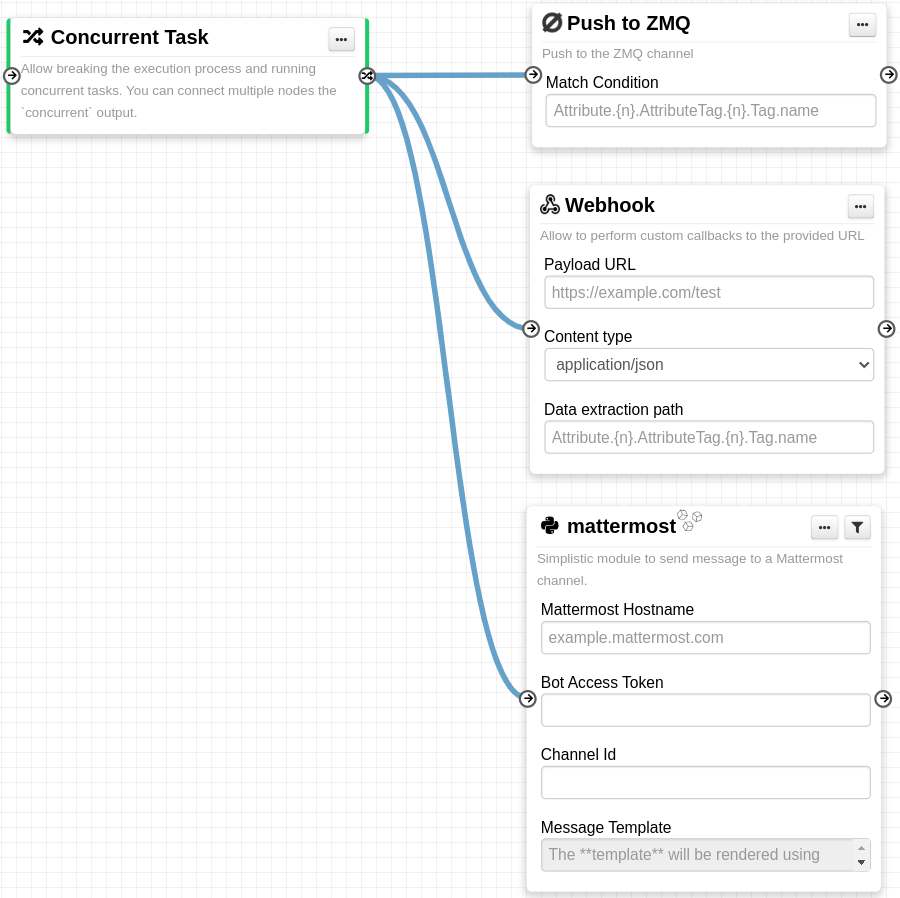
\includegraphics[width=0.5\linewidth]{pictures/module-concurrent.png}}
    \end{center}
\end{frame}

\begin{frame}
    \frametitle{Workflow blueprints}
    \begin{enumerate}
        \item Blueprints allow to \textbf{re-use parts} of a workflow in another one
        \item Blueprints can be saved, exported and \textbf{shared}
    \end{enumerate}
    \begin{center}
        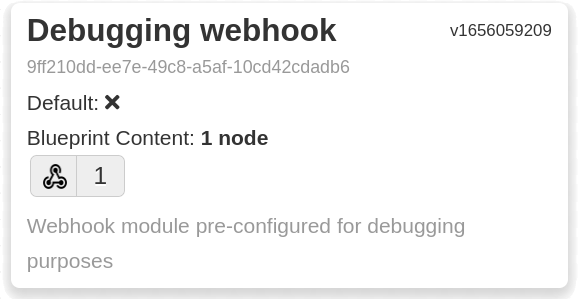
\includegraphics[width=0.5\linewidth]{pictures/blueprint-debugging.png}
    \end{center}
    Blueprints sources: \texttt{\scriptsize MISP/misp-workflow-blueprints} repository\footnote{\scriptsize https://github.com/MISP/misp-workflow-blueprints}
    \begin{itemize}
        \small
        \item Block actions if any attributes have the \texttt{PAP:RED} or \texttt{tlp:red} tag
        \item Curation pipeline
        \item Enrich data from 3rd-party
    \end{itemize}
\end{frame}

\section{Filtering}
\begin{frame}
    \frametitle{Fitlering data on which to apply a module}
    What is the outcome of executing this workflow?
    \begin{center}
        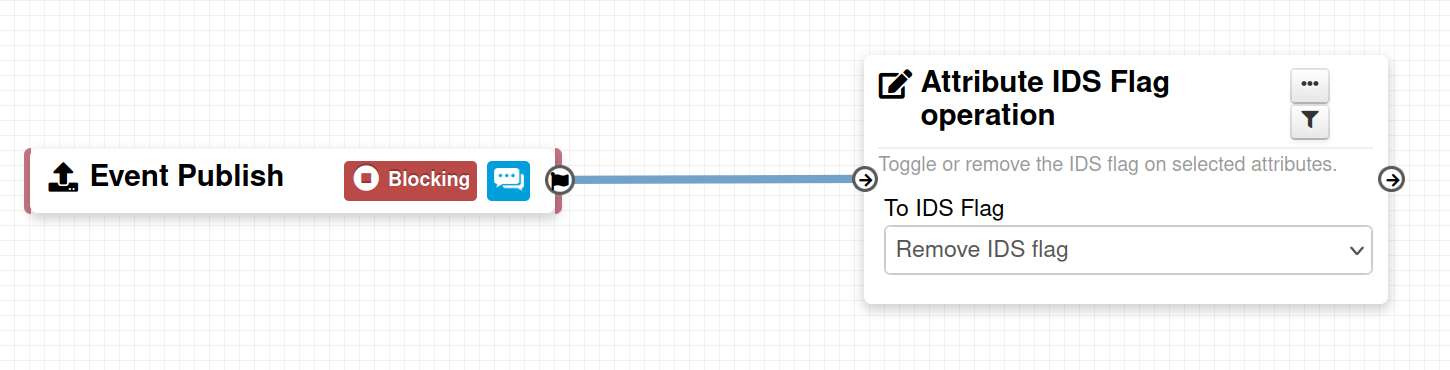
\includegraphics[width=1.0\textwidth]{pictures/remove-ids-1.png}
    \end{center}
    \pause
    \vspace{1em}
    All Attributes get their \texttt{to\_ids} turned off.\\
    \vspace{1em}
    How could we force that action only on Attribute of type \texttt{comment}?
    \begin{center}
        $\rightarrow$ Hash path filtering!
    \end{center}
\end{frame}

\begin{frame}
    \frametitle{Fitlering data on which to apply a module}
    \begin{center}
        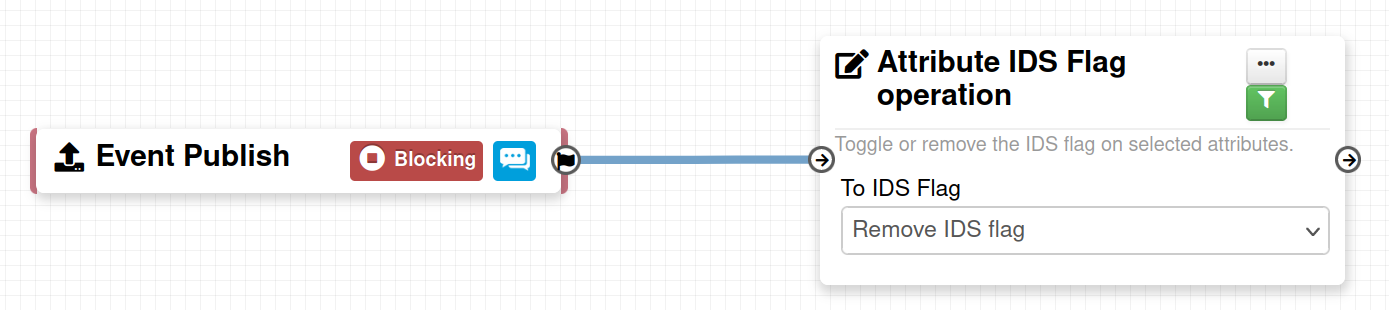
\includegraphics[width=0.5\textwidth]{pictures/remove-ids-3.png}
    \end{center}
    \begin{center}
        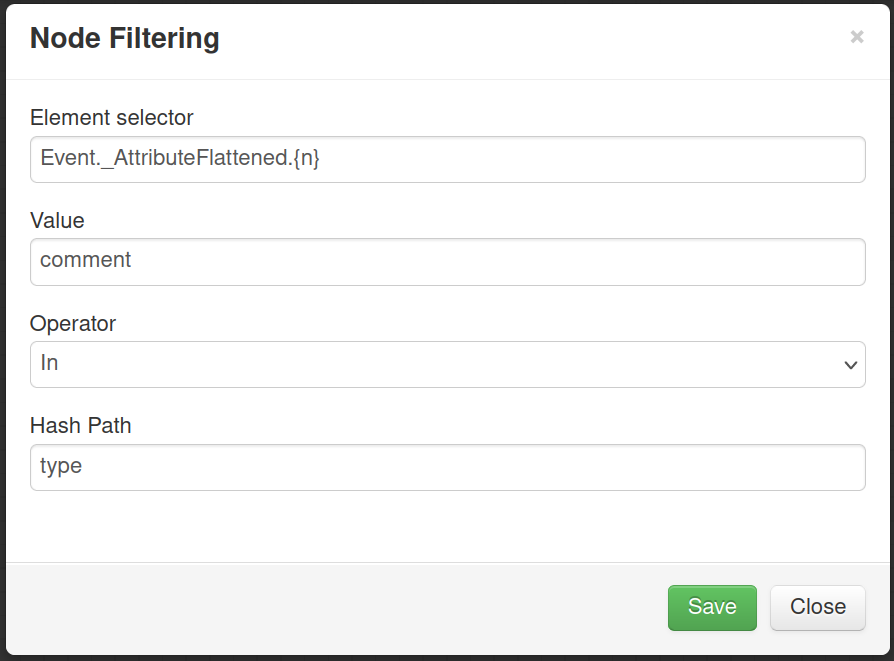
\includegraphics[width=0.9\textwidth]{pictures/remove-ids-2.png}
    \end{center}
\end{frame}

\begin{frame}
    \frametitle{Fitlering data on which to apply a module}
    \begin{center}
        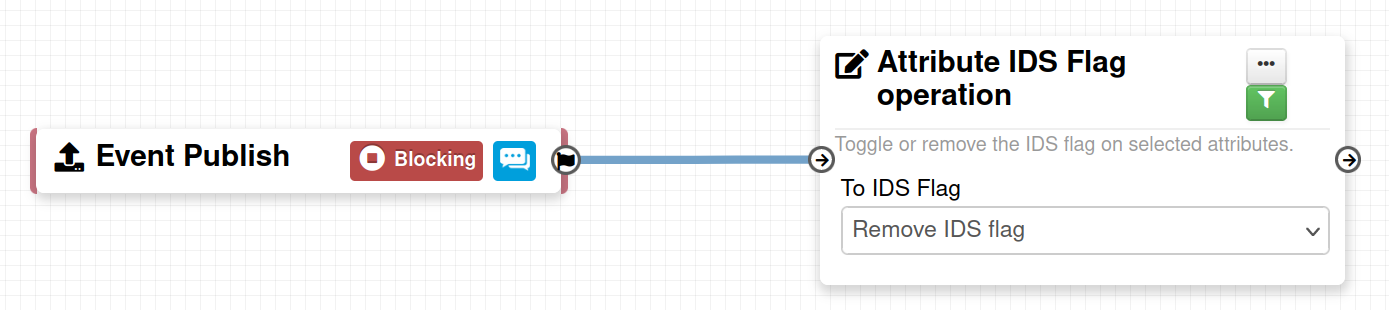
\includegraphics[width=0.5\textwidth]{pictures/remove-ids-3.png}
    \end{center}
    \begin{center}
        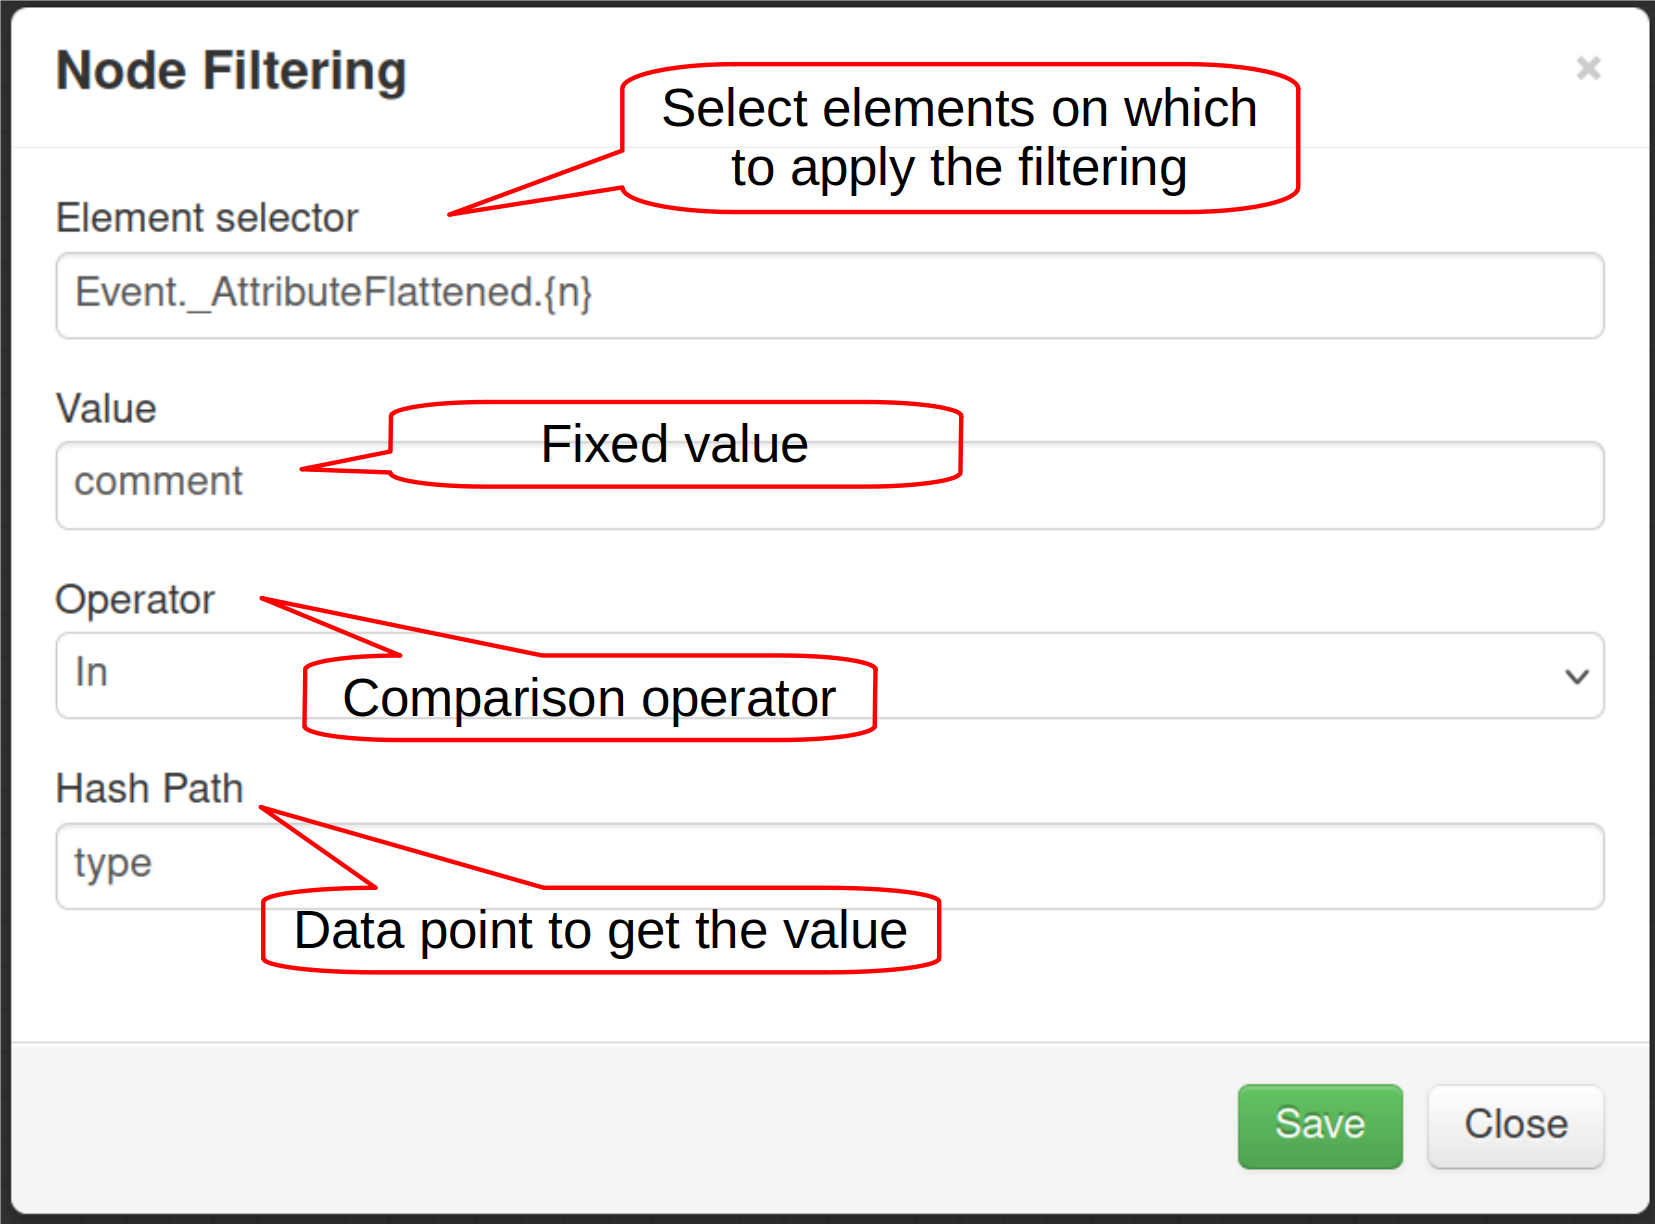
\includegraphics[width=0.9\textwidth]{pictures/remove-ids-2-details.png}
    \end{center}
\end{frame}

\begin{frame}
    \frametitle{Fitlering data on which to apply a module}
    \Wider{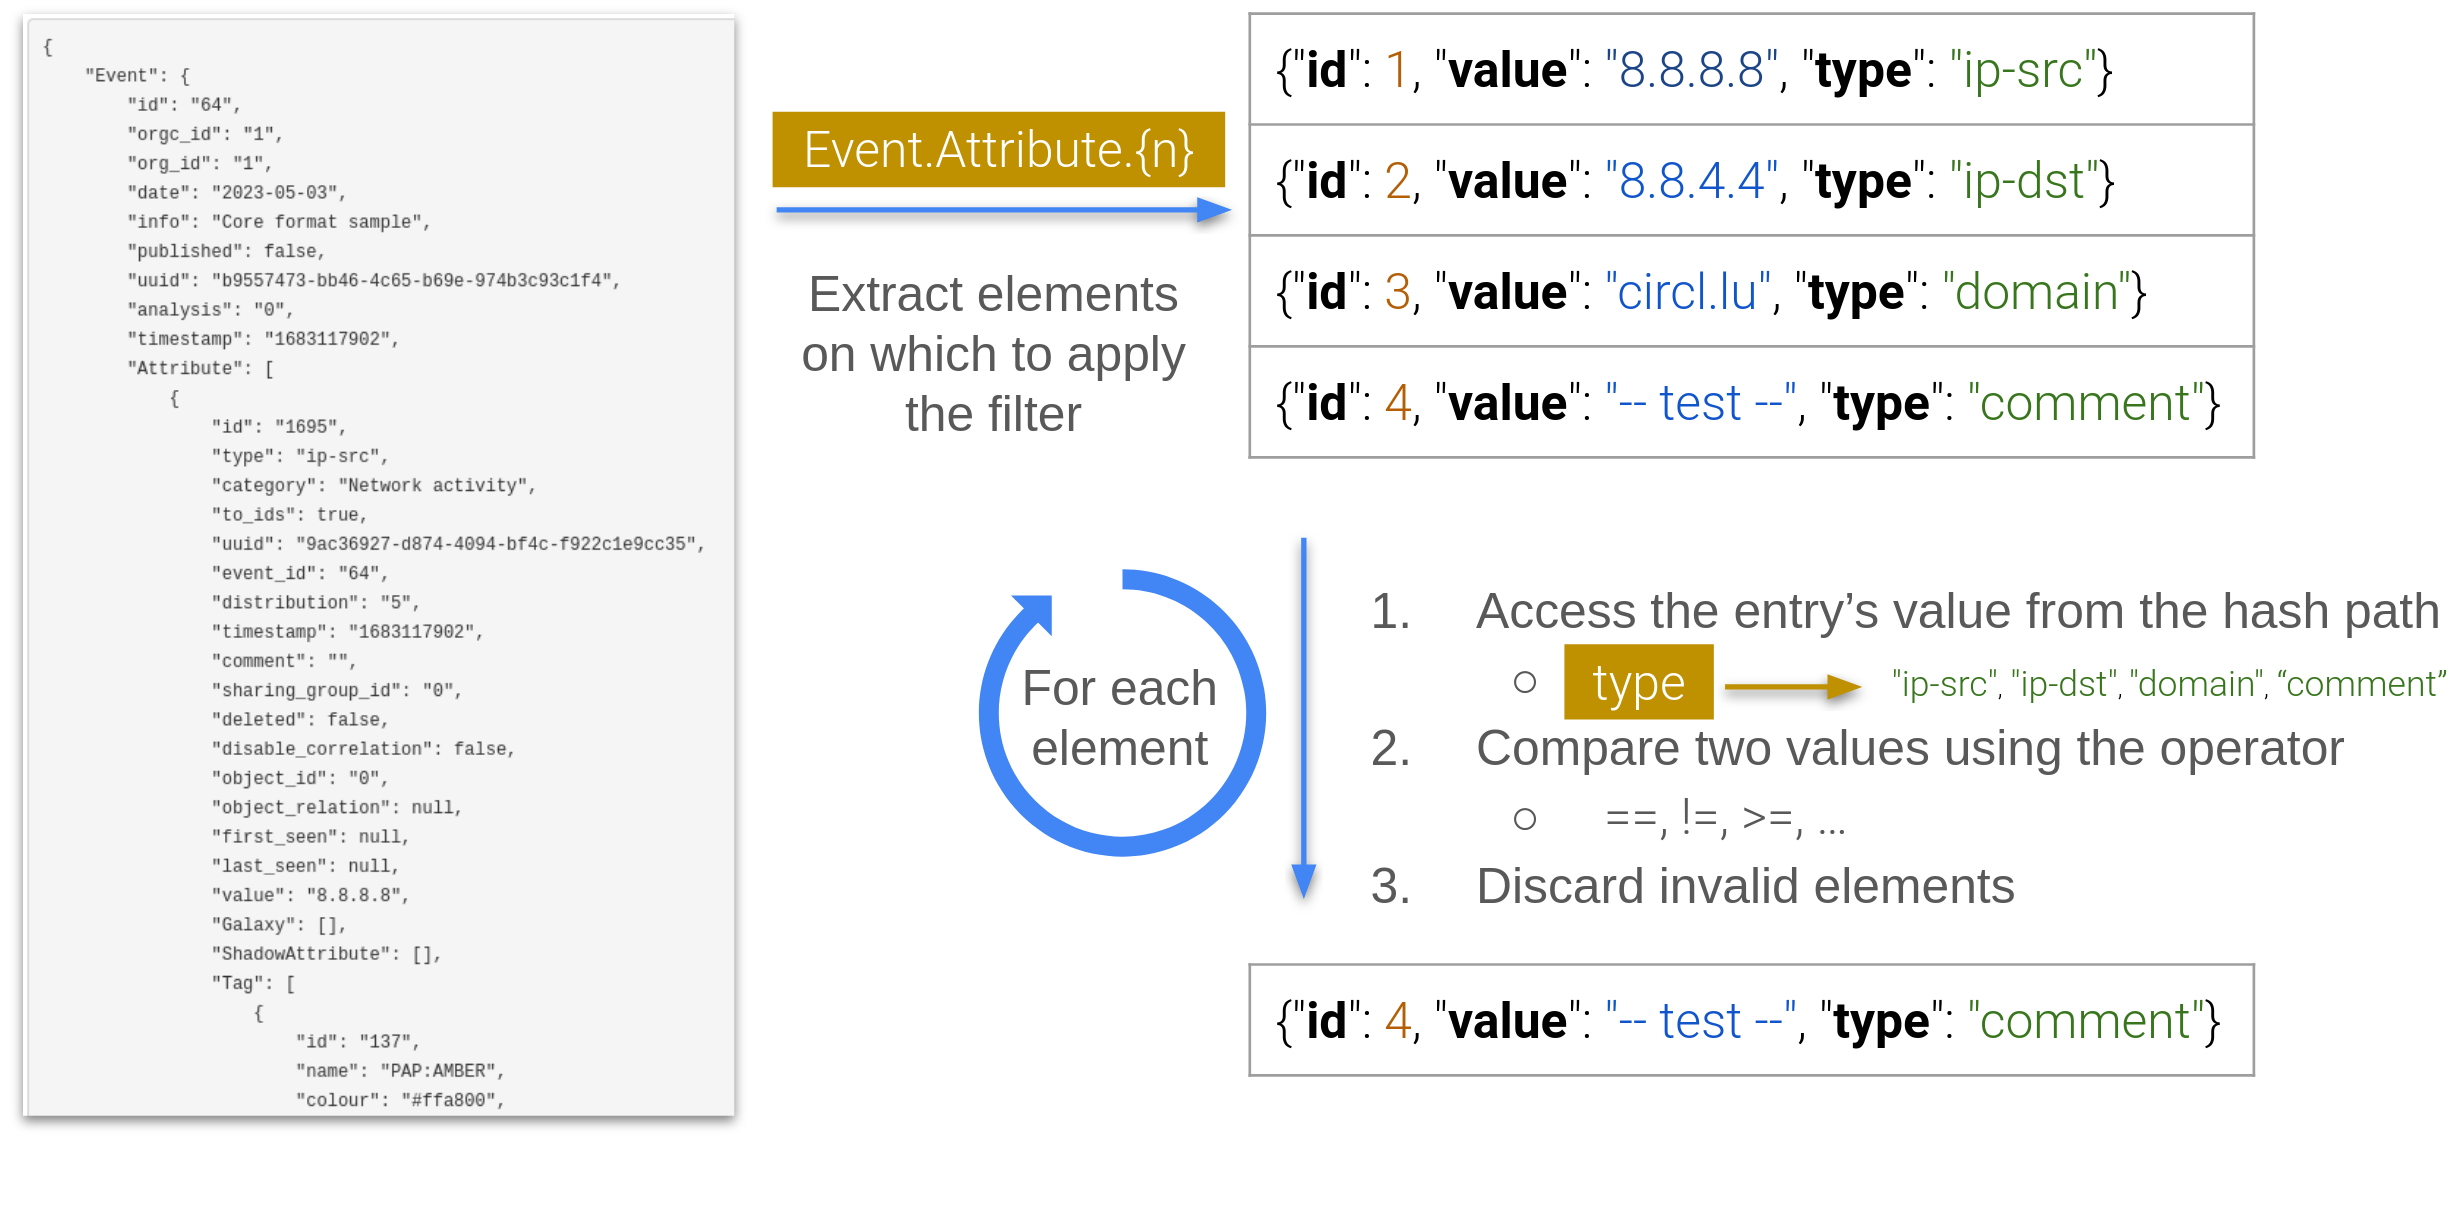
\includegraphics[width=1.01\textwidth]{pictures/filtering-diagram}}
\end{frame}

\begin{frame}
    \frametitle{Fitlering data on which to apply on multiple modules}
    New feature as of \textbf{v2.4.171} allows setting filters on a path.
    \begin{center}
        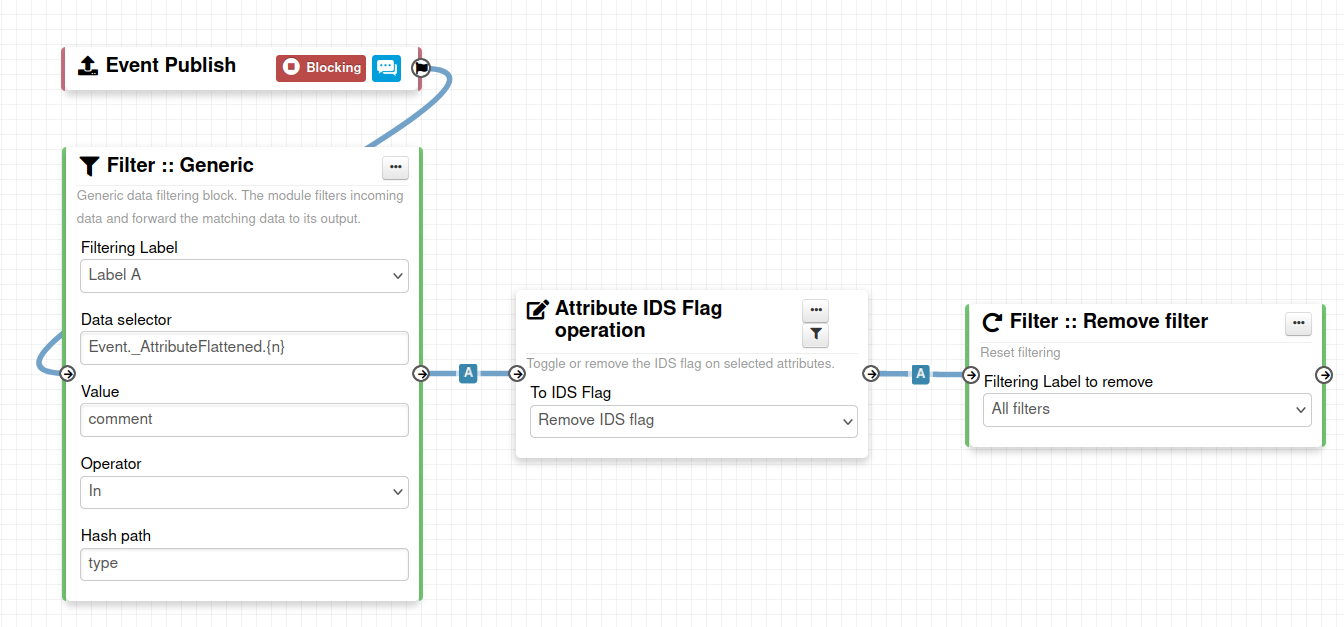
\includegraphics[width=1.0\textwidth]{pictures/remove-ids-generic.png}
    \end{center}
\end{frame}

\begin{frame}
    \frametitle{Data format in Workflows}
    \begin{itemize}
        \item In most cases, the format is the \textbf{MISP Core format}
        \begin{itemize}
            \item Attributes are \textbf{always encapsulated} in the Event or Object
        \end{itemize}
    \end{itemize}
    \begin{center}
        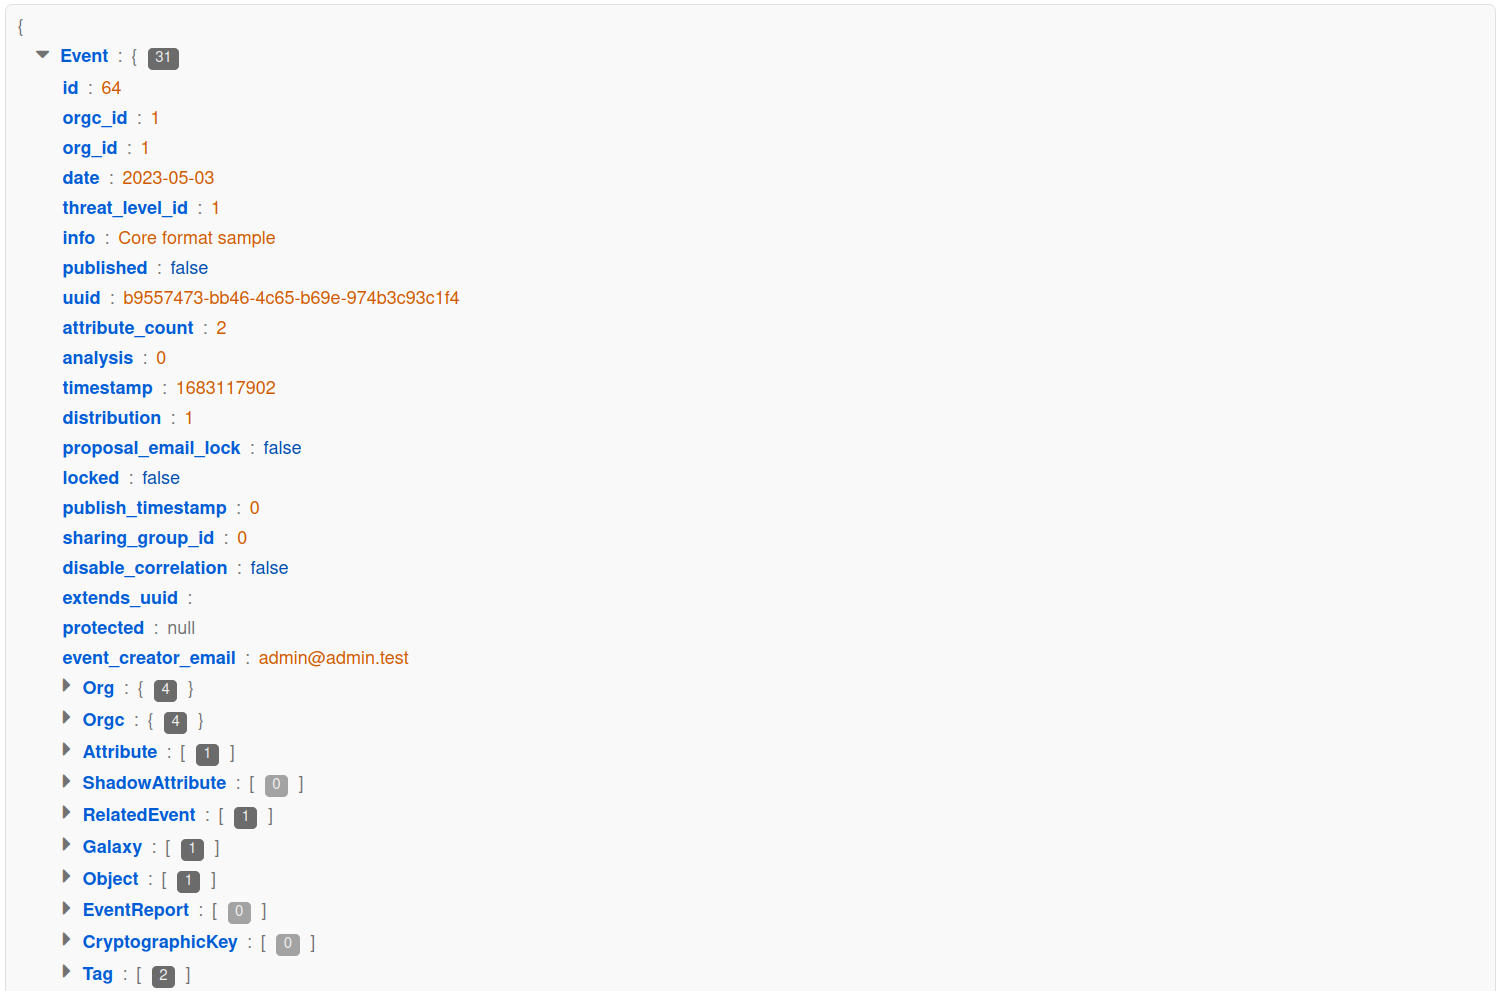
\includegraphics[width=0.9\linewidth]{pictures/misp-core-format.png}
    \end{center}
\end{frame}

\begin{frame}[fragile]
    \frametitle{Hash path filtering - Example}

\begin{lstlisting}[language=javascript,firstnumber=1]
{
    "Event": {
        "uuid": ...
        "timestamp": ...
        "distribution": 1,
        "published": false,
        "Attribute": [
            {
                "type": "ip-src",
                "value": "8.8.8.8", ...
            },
            {
                "type": "domain",
                "value": "misp-project.org", ...
            }
        ],
        ...
    }
}
\end{lstlisting}
    \begin{enumerate}
        \item Access Event distribution
        \begin{itemize}
            \item \texttt{Event.distribution}
        \end{itemize}
    \end{enumerate}
\end{frame}

\begin{frame}[fragile]
    \frametitle{Hash path filtering - Exercise (1)}

\begin{lstlisting}[language=javascript,firstnumber=1]
{
    "Event": {
        "uuid": ...
        "distribution": 1,
        "published": false,
        "Attribute": [
            {
                "type": "ip-src",
                "value": "8.8.8.8", ...
            },
            {
                "type": "domain",
                "value": "misp-project.org", ...
            }
        ],
        ...
    }
}
\end{lstlisting}
    \begin{enumerate}
        \setcounter{enumi}{1}
        \item Access Event published state
        \pause
        \begin{itemize}
            \item \texttt{Event.published}
        \end{itemize}
    \end{enumerate}
\end{frame}

\begin{frame}[fragile]
    \frametitle{Hash path filtering - Exercise (2)}

\begin{lstlisting}[language=javascript,firstnumber=1]
{
    "Event": {
        "uuid": ...
        "distribution": 1,
        "published": false,
        "Attribute": [
            {
                "type": "ip-src",
                "value": "8.8.8.8", ...
            },
            {
                "type": "domain",
                "value": "misp-project.org", ...
            }
        ],
        ...
    }
}
\end{lstlisting}
    \begin{enumerate}
        \setcounter{enumi}{2}
        \item Access all Attribute types
        \begin{itemize}
            \item Hint: Use \texttt{\bf \{n\}} to loop 
            \pause
            \item \texttt{Event.Attribute.\{n\}.type}
        \end{itemize}
    \end{enumerate}
\end{frame}

\begin{frame}[fragile]
    \frametitle{Hash path filtering - Exercise (3)}

\begin{lstlisting}[language=javascript,firstnumber=1]
{
    "Event": {
        "Attribute": [
            {
                "type": "ip-src",
                "value": "8.8.8.8",
                "Tag": [
                    {
                        "name": "PAP:AMBER", ...
                    }
                ], ...
            }
        ],
        ...
    }
}
\end{lstlisting}
    \begin{enumerate}
        \setcounter{enumi}{2}
        \item Access all Tags attached to Attributes
        \pause
        \begin{itemize}
            \item \texttt{Event.Attribute.\{n\}.Tag.\{n\}.name}
        \end{itemize}
    \end{enumerate}
\end{frame}


\begin{frame}[fragile]
    \frametitle{Hash path filtering - Exercise (4)}

\begin{lstlisting}[language=javascript,firstnumber=1]
{
    "Event": {
        "Tag": [
            {
                "name": "tlp:green", ...
            }
        ], ...
        "Attribute": [
            {
                "value": "8.8.8.8",
                "Tag": [
                    {
                        "name": "PAP:AMBER", ...
                    }
                ], ...
            }
        ],
    }
}
\end{lstlisting}
    \begin{enumerate}
        \setcounter{enumi}{3}
        \item Access all Tags attached to Attributes and from the Event
        \begin{itemize}
            \item Hint: Use \texttt{\bf \_allTags} to access {\bf all} tags
        \end{itemize}
    \end{enumerate}
\end{frame}

\begin{frame}[fragile]
    \frametitle{Hash path filtering - Exercise (4)}

\begin{lstlisting}[language=javascript,firstnumber=1]
{
    "Event": {
        "Tag": [
            {
                "name": "tlp:green", ...
            }
        ], ...
        "Attribute": [
            {
                "value": "8.8.8.8",
                "Tag": [
                    {
                        "name": "PAP:AMBER", ...
                    }
                ], ...
            }
        ],
    }
}
\end{lstlisting}
    \begin{enumerate}
        \setcounter{enumi}{3}
        \item Access all Tags attached to Attributes and from the Event
        \begin{itemize}
            \item \texttt{Event.Attribute.\{n\}.\_allTags.\{n\}.name}
        \end{itemize}
    \end{enumerate}
\end{frame}

\begin{frame}[fragile]
    \frametitle{Hash path filtering - Exercise (4)}

\begin{lstlisting}[language=javascript,firstnumber=1]
{
    "Event": {
        "Tag": [...],
        "Attribute": [
            {
                "value": "8.8.8.8",
                "_allTags": [
                    {
                        "name": "tlp:green",
                        "inherited": true, ...
                    },
                    {
                        "name": "PAP:AMBER",
                        "inherited": false, ...
                    }
                ],
            }
        ...
}
\end{lstlisting}
    \begin{enumerate}
        \setcounter{enumi}{3}
        \item Access all Tags attached to Attributes and from the Event
        \begin{itemize}
            \item \texttt{Event.Attribute.\{n\}.\_allTags.\{n\}.name}
        \end{itemize}
    \end{enumerate}
\end{frame}

\begin{frame}
    \frametitle{Data format in Workflows}
    \begin{center}
        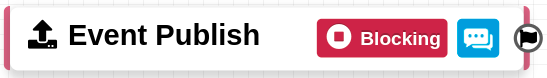
\includegraphics[width=0.7\linewidth]{pictures/workflow-trigger.png}
    \end{center}
    \begin{itemize}
        \item In most cases, the format is the \textbf{MISP Core format}
        \begin{itemize}
            \item Attributes are \textbf{always encapsulated} in the Event or Object
        \end{itemize}
        \item The MISP Core format has \textbf{additional properties}
        \begin{itemize}
            \item Additional key \textbf{\texttt{\_AttributeFlattened}}
            \item Additional key \textbf{\texttt{\_allTags}}
            \item Additional key \textbf{\texttt{inherited}} for Tags
        \end{itemize}
    \end{itemize}
\end{frame}

\section{Debugging}
\begin{frame}
    \frametitle{Debugging Workflows: Log Entries}
    \begin{itemize}
        \item Workflow execution is logged in the application logs:
        \begin{itemize}
            \item \texttt{/admin/logs/index}
            \item \faIcon{exclamation-triangle} Might be phased out as its too verbose
        \end{itemize}
        \item Or stored on disk in the following file:
        \begin{itemize}
            \item \texttt{/app/tmp/logs/workflow-execution.log}
        \end{itemize}
    \end{itemize}
    \begin{center}
        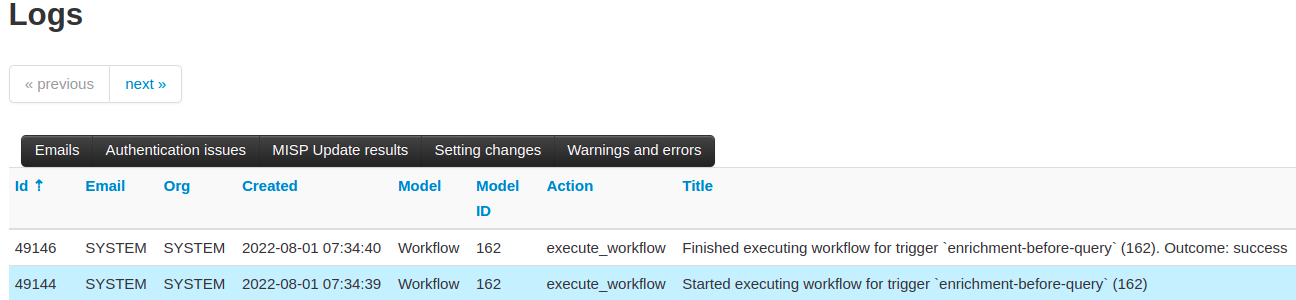
\includegraphics[width=1.0\linewidth]{pictures/workflow-debug.png}
    \end{center}
\end{frame}

\begin{frame}
    \frametitle{Debugging Workflows: Debug mode}
    \begin{itemize}
        \item The 
\includegraphics[width=70px]{pictures/debug-mode.png} can be turned on for each workflows
        \item Each nodes will send data to the provided URL
        \begin{itemize}
            \item Configure the setting: \texttt{Plugin.Workflow\_debug\_url}
        \end{itemize}
        \item Result can be visualized in
        \begin{itemize}
            \item \textbf{offline}: \texttt{tools/misp-workflows/webhook-listener.py}
            \item \textbf{online}: \url{requestbin.com} or similar websites
        \end{itemize}
    \end{itemize}
    \begin{center}
        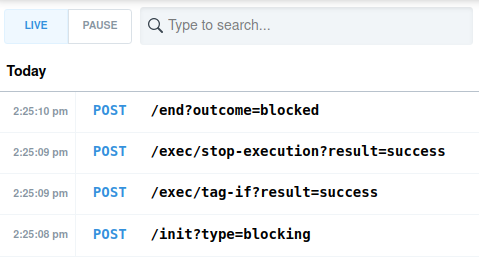
\includegraphics[width=0.6\linewidth]{pictures/request-bin.png}
    \end{center}
\end{frame}

\begin{frame}
    \frametitle{Debugging modules: Re-running workflows}
    \begin{itemize}
        \item Try workflows with custom input
        \item Re-run workflows to ease debugging
    \end{itemize}
    \begin{center}
        \frame{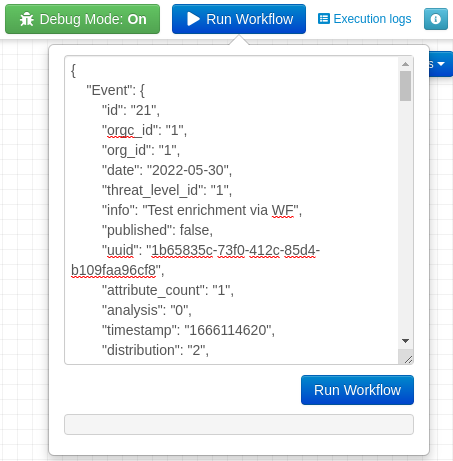
\includegraphics[width=0.55\linewidth]{pictures/running-workflows.png}}
    \end{center}
\end{frame}

\begin{frame}
    \frametitle{Debugging options}
    \begin{itemize}
        \item Workflow \textbf{execution and outcome}
        \item Individual module \textbf{execution and outcome}
        \item \textbf{Live} workflow debugging with module inspection
        \item \textbf{Re-running/testing} workflows with custom data
    \end{itemize}
\end{frame}

\begin{frame}
    \frametitle{Should I migrate to MISP Workflows}
    I have automation in place using the API/ZMQ. Should I move to Workflows?
    \vspace{1em}
    \begin{itemize}
        \item I have a curation pipeline using the API, should I port it to workflows?
        \begin{itemize}
            \item \textbf{No} in general, but WF can be used to start the curation process or perform simple pre-processing
        \end{itemize}
        \item What if I want to \textbf{block} some actions
        \begin{itemize}
            \item Put the blocking logic in the WF, keep the remaining outside
        \end{itemize}
        \item Bottom line is \textbf{Keep it simple} for you to maintain
    \end{itemize}
\end{frame}

\begin{frame}
    \frametitle{Future works}
    \begin{itemize}
        \item More action modules 
\includegraphics[width=12px]{pictures/sc-action-icon.png}
        \item More logic modules 
\includegraphics[width=12px]{pictures/sc-condition-icon.png}
        \item More triggers 
\includegraphics[width=12px]{pictures/sc-event-icon.png}
        \item Recursion prevention system
        \item Improvement for logging
    \end{itemize}
\end{frame}

\begin{frame}
    \frametitle{Final words}
    \begin{itemize}
        \item Designed to \textbf{quickly} and \textbf{cheaply} integrate MISP in CTI pipelines
        \item Waiting for feedback!
        \begin{itemize}
            \item New triggers?
            \item New modules?
        \end{itemize}
    \end{itemize}
\end{frame}

